\documentclass{article}
\usepackage[T1]{fontenc}
\usepackage{graphicx}
\graphicspath{ {../img/} }

\begin{document}
    \title{Laboratorium Podstawy Aplikacji Internetowych \\
    Spring}
    \author{Piotr Tylczyński \\
    \texttt{piotr.tylczynski@ptl.cloud}}
    
    \begin{titlepage}
        \maketitle
    \end{titlepage}
    
    \tableofcontents
    \pagebreak
    
    \section{Wstęp}
    Celem tego laboratorium jest pokazanie działanie frameworku Spring w praktyce. Podczas zajęć wykonasz prosty serwer, który obsłuży API dla wypożyczalni samochodów. \\
    Stworzone przez ciebie rozwiązanie będzie bardzo uproszczone w porównaniu do prawdziwych serwerów jakie obsługiwały by takie zadanie. Jednak nie oznacza to że będzie bezużyteczne. Nie licząc braku systemu autoryzacji, stworzysz serwer zgodnie z aktualnymi standardami produkcji takich systemów.
    
    \section{Założenia projektu}
        Tworzymy prosty serwer backendowy służący do obsługi wyporzyczalni samochodów. Chcielibyśmy móc dodawać i usuwać samochody z naszej wyporzyczalni. Oczywiście nie powinno się to dziać zawsze, ale tylko wtedy kiedy nikt z nich nie korzysta - szczególnie ważne w momencie gdy mówimy o usuwaniu auto ze stanu wyporzyczalni. \\
        Dodatkową opcją będzie śledzenie kto, kiedy i co wyprzyczył. Z tego powodu będziemy musieli stworzyć bazę danych klientów.
    
    \section{Inicjalizacja projektu}
        Całość tworzenia kodu rozpoczniemy od stworzenia projektu. W tym celu mamy dwa wyjścia. W pierwszym możemy ręcznie szukać odpowiednich modułów Springa w internecie i repozytoriach \emph{Mavena}. W drugim skorzystamy z rozwiązania Spring Initializr. Trzymając się założeń, że korzystamy z rowiązań wykorzystywanych w przemyśle skorzystamy z Initializr. \\
        Initializr został stworzony w 2013 roku przez firmę VMware, Inc. i jest prostą aplikacją służącą do szybkiego tworzenia baz dla projektów Springa. Możemy w nim wybrać interesujące nas moduły a aplikacja sama zajmie się wyszukaniem ich w repozytoriach Maven i dodaniem odpowiednich wpisów w \emph{pom.xml} jaki i stworzeniem odpowiednich plików w samym projekcie. \\
        Osoby chętne mogą same skorzystać z Initializr i przejść przez kreator. W tym celu należy wskazać moduły:
        \begin{itemize}
            \item Lombok
            \item Spring Web
            \item Spring Data JPA
            \item H2 Database
        \end{itemize}
        Zachęcam jednak do pobrania gotowego prekonfigurowanego repozytorium z linku na końcu skryptu. Pomoże to w uniknięciu prostych błędów i rozbierzności w samej konfiguracji projektu. \\
        Ważnym elementem do rozważenia na tym etapie jest struktura projektu. Spring nie narzuca nic konkretnego, jednak skorzystamy z podejścia jedna funkcjinalność, jeden folder. Pomoże to nam w przyszłości szybko nawigować się po projekcie. Szczególnie jeśli kiedyś zdecydujemy się na jego rozwijanie. Zastanówmy się teraz jakie funkcjonalności mamy do zaimplementowania. Na pewno jest to element zajmujący się klientami, oraz element zajmujący się klientami. Z tego powodu stworzymy dwa foldery. Jeden dedykowany dla kodu obsługującego logikę kilentów i jeden dla logiki aut.
        
        \begin{figure}[h]
            \centering
            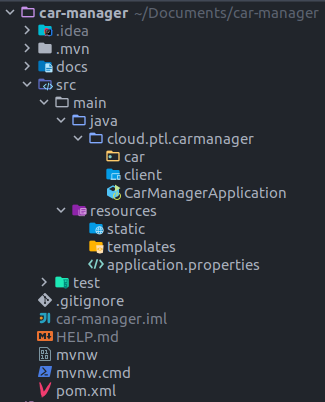
\includegraphics{tree.png}
        \end{figure}
    
    \section{Modelowanie Bazy Danych}
        Najprostszym, jednak bardzo nie efektywnym sposobem będzie ręczne stworzenie schematu bazy danych przez podawanie odpowiednich komend SQL. Następnie do obsługi takiej bazy danych użylibyśmy biblioteki JDBC, tak jak było to pokazywane na zajęciach z Systemów Baz Danych podczas 5 semestru. Jednak jak wspomniałem na początku jest to podejście bardzo nie efektywne. Wyobraźmy sobie, że zamiast modelowania tylko dwóch elementów chcielibyśmy stworzyć ich dwadzieścia. Być może stworzenie bazy danych nie byłoby wyzwaniem, jednak stworzenie i zarządanie skryptami JDBC już tak. Dalej byłoby jeszcze gorzej, ponieważ bazę danych od czasu do czasu trzeba zmieniać, zgodnie ze zmieniającymi się wymaganiami projektu, a to niesie ze sobą potrzebe ręcznego przemodelowania bazy danych a to zmianę skryptów. A na końcu musimy pamiętać, że wiele baz danych posiada swoje charakterystyczne dialekty, co wcale nie ułatwia tworzenia agnostycznego kodu. \\
        Z tego powodu skorzystamy z jednego z modułów, który sami dodaliśmy - Spring Data. Jest to moduł, który za pomocą standardu JPA - Java Persistence API - oraz projektu Hobernate pozwala na modelowanie bazy danych jako obiektów Javy. Hibernate jest tak zwanym ORMem - Object Relation Mapper. W ten sposób możemy całkowicie zapomnieć o pisaniu czegokolwiek samemu. Od teraz będziemy tworzyć obiekty POJO i odpowiednio je oznaczać a Hibernate zrobi wszystko za nas.
        
        \subsection{Obiekty POJO}
            \textbf{POJO} - Plain Old Java Object.\\
            POJO to tak naprawdę obiekty, które powinny składać się tylko i wyłącznie z pól, getterów i setterów. Oczywiście, my napiszemy tylko definicje pól a resztę zrobi za nas projekt Lombok. Dodatkowo będziemy musieli odpowiednio oznaczyć poszczególne pola tak, żeby Hibernate wiedział co i jak ma utrwalać w bazie danych.
\end{document}